%% intro.tex

\section{Introduction}
\label{sec:intro}

  In this paper, we study efficient enumeration of classes of unusual words in a string.
  %% In this paper, we study efficient enumeration of non-trivial MAWs and other classes of unusual words, such as the \textit{minimal unique substrings} (MUSs) and the \textit{minimal rare words} (MRWs) in a string.
  A \textit{minimal absent word} (MAW) of a string $S$ is a string $w$ that does not occur in $S$ and any proper substring of $w$ occurs in $S$ as a substring. For any integer $k\ge 0$, as most general form of unusual word, a \textit{minimal rare word} (MRW) of $S$ with frequency $k$ is any string $w$ that occurs in $S$ exactly $k$ times, and any proper substring of $w$ has strictly less occurrences in $S$. An unusual word is said to be non-trivial if it has length at least two.
Presently, most practical algorithms for unusual words use the suffix array or the Burrows-Wheeler transform of $S$ rather than space inefficient data structures such as the suffix trees. However, all the previous algorithms for MAWs, MUSs, and MRWs have the total amount of time that grows linearly in the length $n$ of $S$.
  In this paper, we present a new algorithm that, based on the suffix and the inverse suffix arrays, longest common prefix array, and an input text, computes the set $MAW(S)$ of all minimal absent words in a string $S$. The algorithm runs in $O(e_R + occ)$, where $occ$ denotes the number $|MAW(S)|$ of solusions, and  $e_R$ denotes the number of right-extensions of maximal repeats in $S$. For any string $S$ of length $n$, $e_R$ is linear in $n$, and can be sublinear in $n$, up to logarithmic.
  We also show that modified algorithms computes \textit{minimal unique substrings} (MUSs) and their generalization, called \textit{mininimal rare words} (MRWs), in similar time complexities. 

%% \textbf{Backgrounds}.\ 
%% %%%%%
%% \textit{Enumeration of maximal repeats} in a string is one of the most important problems in string processing and bioinfomatics, and has been extensively studied for decades since their discovery~\cite{blumer1987complete,crochemore:verin1997compact,raffinot2001maximal}. 
%% A \textit{maximal repeat} (MR) is such a substring of a string that occurs at least twice and cannot be extended to the left or to the right without losing their occurrences. 
%% This paper studies the problem of enumerating \textit{all distinct maximal repeats} in a string of length $n$ using the suffix array $SA$~\cite{manber:myers1993suffixarrays} and associated auxiliary structures, following the direction of the literature~\cite{narisawa2007efficient,okanohara2009text,beller:berger2012space:efficient:bbo,belazzougui2020linear,nishimoto:cpm2021enum}.

%% Fundamental parameters related to this problem are the numbers $\mu = \mu(S)$ and $e_R = e_R(S)$ of maximal repeats and their \textit{right extensions} in a string $S$, respectively, satisfying that $\mu \le e_R\le n$.
%% %The parameter $e_R$ was introduced by \cite{belazzougui:cunial:gagie:prezza:raffinot2015composite} as for measuring the repetitiveness of a text. 
%% Especially, the $e_R(S)$ was introduced by Belazzougui~\textit{et al.}~\cite{belazzougui:cunial:gagie:prezza:raffinot2015composite} as one of the fundamental parameters to measure the repetitiveness of a string, which upperbounds other parameters $r(S)$ (the number of \textit{BWT runs}) and $z(S)$ (the number of \textit{LZ-phrases})~\cite{belazzougui:cunial:gagie:prezza:raffinot2015composite}, and is known to be much smaller than the string length $n$, even logarithmically, for highly-repetitive strings~\cite{radoszewski:rytter2012structure:cdawg:thuemorse}. Hence, we aim at divising an efficient algorithm whose time and space complexities are sensitive to the repetitiveness parameter $e_R$. 
%% To help enumeration, we allow to use the following linear space auxiliary structures as black box: the inverse SA ($ISA$), the input string ($S$), and the \textit{range minima query} ($RMQ$) structure built on the \textit{longest common prefix} ($LCP$) array, easily built from $SA$, on which each maximal repeat is encoded in $O(1)$ size (see \cref{sec:triple}). 

%% %%where there are at most $n$ distinct maximal repeats in the input length $n$~\cite{blumer1987complete,raffinot2001maximal}.

%% %% We consider the problem of enumerating \textit{all distinct maximal repeats} in a string of length $n$ in sublinear time , where there are at most $n$ distinct maximal repeats in the input length $n$~\cite{blumer1987complete,raffinot2001maximal}.

%% %%%%%%%%
%% %% %%%%
%%%%%%
\begin{figure}[t]
\centering  
\includegraphics[width=1.00\textwidth]{fig/exp1/fwdstree-crop.pdf}
\smallskip
  \caption{Illustration of the search strategies for maximal repeat enumeration. The figure shows two search trees for a string $S = \mathtt{\#abcadabcabc\$}$ of \cref{tbl:arrays}: the black tree is the suffix tree of $S$; the red tree is the Winer tree of $S$. In the trees, each circle indicates a node with a right-branching substring as its string label, each double black-red circle indicates a maximal repeat, and each cross a locus on an edge. To each node, its SA-range $[L..R]$ or $[L]$ in \cref{tbl:arrays} is attached. 
    Note that each black edge has a string label of length one or more, while each red edge has a character label of length one.
    The previous algorithms \BUSA{} and \TDBW{} in in \cref{sec:prev} traverses the entire black subtree of $\Theta(n)$ nodes bottom-up (\cref{rem:lb:busa}) and red subtree of $\Theta(n)$ nodes top-down (\cref{rem:lb:tdbw}), while the proposed \TDSA{} in \cref{sec:algo} traverses only $\mu$ red nodes following $O(e_R)$ black edges (\cref{lem:prune:leftbranch}). $\diamond$
    %% \BUSA{} and \TDSA{} traverse the black subtree bottom-up and top-down, resp., while \TDBW{} traverses the red subtree top-down. 
}\label{fig:fwdstree}
\end{figure}
%%%%%%


%% %%%%%%
%% \begin{figure}[t]
%% \centering  
%% %% \includegraphics[width=1.00\textwidth]{fig/exp1/fwdstree-crop.pdf}
%% 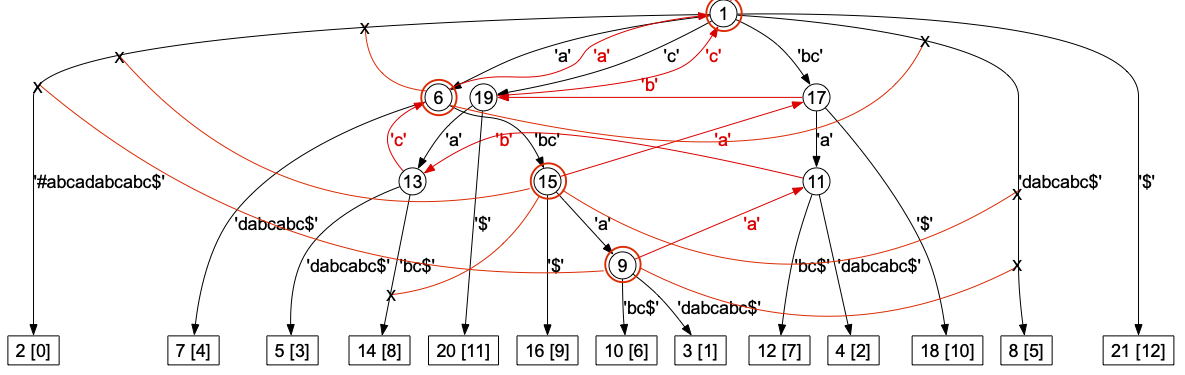
\includegraphics[width=1.00\textwidth]{fig/exp1/fwdstree_org.png}
%% \smallskip
%% \caption{
%%   Illustration of search strategies for maximal repeat enumeration on a string
%%   $S = \mathtt{\#abcadabcabc\$}$ of \cref{tbl:arrays}. 
%%   %S=#abcadabcabc$.
%%   The figure shows the suffix tree (black) and Winer tree (red) of $S$, highlighting maximal repeats with red double circles. Nodes represent right-branching substrings labeled with its SA-range, and edges are labeled with strings (black) or characters (red). Previous methods $\BUSA$ and $\TDBW$ traverse entire subtrees, while our method $\TDSA$ efficiently traverses only relevant red nodes via black edges, significantly reducing the search space.
%% }\label{fig:fwdstree}
%% \end{figure}
%% %%%%%%


%% %%%%%%%%

%% \textbf{Previous work}.\ 
%% %%%%%
%% The current best upperbounds on the runtime of enumerating all distinct  maximal repeats were summarized as the following algorithm schema (see \cref{fig:fwdstree}).
%% The first scheme is abbreviated as \BUSA{} (bottom-up search with the suffix array),  and the best runtime was $O(n)$ time using $O(n)$ words of space based on $SA$, $ISA$, and the RMQ structure on $LCP$, shown by Narisawa, Inenaga, Bannai, and Takeda~\cite{narisawa2007efficient}. 
%% The second scheme is abbreviated as \TDBW{} (top-down search with the Burrows-Wheeler Transformation/BWT), and the runtime was $O(n \log\sigma)$ time using $O(n/\log_\sigma n)$ words of space based on the Wavelet tree on $BWT$, shown by Beller, Berger, and Ohlebusch~\cite{beller:berger2012space:efficient:bbo}.
%% %%where $ISA$ is the inverse $SA$, and $LCP$ is the longest common prefix array of the string.
%% After these seminal work with \textit{uncompressed indexes}~\cite{narisawa2007efficient,beller:berger2012space:efficient:bbo}, there have been a few recent researches on repetition-aware enumeration of maximal repeats with \textit{compressed indexes}~\cite{belazzougui2020linear,nishimoto:cpm2021enum}. For example, Nishimoto and Tabei~\cite{nishimoto:cpm2021enum} have nicely reduced the space to $O(r(S))$ with polylogarithmic factor retaining $O(n)$ time based on a variant of the \textit{$r$-index}. However, to the best of our knowledge, there have been no results that simutaneously achieve sublinear space and time sensitive to repetition parameters including $r(S), z(S)$, or $e_R(S)$. 


%% %%%%%%% tblnew.tex
%% %%% tabnew.tex
%% %\centering
%% \begin{table}[t]
%%   \caption{%
%%     Summary of the time and space of the previous and proposed algorithms for enumeration of all distinct maximal repeats in a string $S$ of length $n$,
%%     %of maximal repeats,
%%     %% where $\sigma$ is the alphabet size,
%%     %% $r$ is the number of BWT runs,
%%     %% $e_R$ is the number of right-extensions,
%%     %% %of maximal repeats,
%%     where
%%     $\sigma$, $r$, and $e_R$ are the numbers of 
%%     characters, BWT runs, and right-extensions, respectively, 
%%     $\delta$ is the substring complexity of $S$.
%%     See \cref{sec:prelim:ds:array} for abbreviations in column \textit{Data structure}, and BU/TD and SA/BW indicate bottom-up/top-down search and SA/BWT arrays, respectively, in \textit{Scheme}.
%% }\label{table:summary:new}
%% %%%% 
%% \medskip
%% \begin{minipage}{\textwidth}
%% %\hspace{-1.2em}
%% \begin{tabular}{%
%% p{.0em}%1margin
%% p{7.6em}%2algo
%% p{10.0em}%3underlying
%% >{\centering}p{7em}%5time
%% %>{\centering}p{8.5em}%6indexspace
%% >{\centering}p{8.5em}%%6indexspace
%% p{3.0em}%4type
%% %c%7dammy
%% %>{}p{4.9em}%7dammy
%% }\toprule
%%   & Algorithm
%%   & Data Structure	
%%   %% & Underlying\break Structure	
%% %% & Index Space
%% & Space (words)
%% & Enum.~Time 
%% & Scheme \\
%% %%%%
%% \midrule 
%% %% \multicolumn{6}{l}{Existing array-based algorithms} \\
%% & Narisawa~\cite{narisawa2007efficient}	&
%% \textsc{Sa,\,Isa,\,Txt,\,Lcp}\cite{manber:myers1993suffixarrays} & $O(n)$	& $O(n)$ & \BUSA{} 	 \\
%% %% & Narisawa~\cite{narisawa2007efficient}	& SA\cite{manber:myers1993suffixarrays} & $O(n)$	& $O(n)$ & \BUSA{} 	 \\
%% %% & Okanohara+~\cite{okanohara2009text}	& SA\cite{manber:myers1993suffixarrays}\&FM\cite{Ferragina05:FM} & $O(n)$& $O(n\log\sigma)$	 & \bufwd 	 \\
%% & Beller+~\cite{beller:berger2012space:efficient:bbo} 	&
%% \textsc{Bwt,\,Wt}~\cite{Ferragina05:FM}
%% & $O(n/\log_\sigma n)$ & $O(n\log\sigma)$	& \TDBW{} \\
%% & Belazzougui+\cite{belazzougui2015space:unusual} 	&
%% \textsc{Bwt,\,Rdq}~\cite{belazzougui2020linear}
%% & $O(n/\log_\sigma n)$ & $O(n)$	& \TDBW{} 	 \\
%% %% & Belazzougui+\cite{belazzougui2020linear} 	& Belazzougui+\cite{belazzougui2020linear} & $O(n)$ & $O(n)$	& \TDBW{} 	 \\
%% %% & Belazzougui+\cite{belazzougui2020linear} 	& Belazzougui+\cite{belazzougui2020linear} & $O(n\log n\log\sigma)$ & $O(n)$	& \TDBW{} 	 \\
%% & Nishimoto+~\cite{nishimoto:cpm2021enum} 	& Gagie+~\cite{gagie:navarro:prezza2020fully} & $O(r\log({\frac n r})\log n)$ & $O(n\polylog n)$ & \TDBW{} 	 \\
%% %%%%%
%% %% \multicolumn{6}{l}{Proposed algorithms} \\
%% \\
%% & [This paper]	&
%% \makebox[11em][l]{\textsc{Sa,\,Isa,\,Txt,\,Rmq$_\textsc{LCP}$}\!\cite{manber:myers1993suffixarrays}}
%%  & $O(n)$ & $O(e_R)$	& \TDSA	 \\
%% %% & [This paper]	& SA\cite{manber:myers1993suffixarrays} & $O(n)$ & $O(e_R)$	& \TDSA	 \\
%% & [This paper]   	& Gagie+~\cite{gagie:navarro:prezza2020fully}	 	& $O(r\log({\frac n r})\log n)$ & $O(e_R \log({\frac n r}))$& \TDSA \\
%% & [This paper]   	& $\delta$-SA~\cite{kempa:kociumaka2023collapsing}  & $O(\delta\log({\frac n \delta}) \log n)$	& $O(e_R \log^{4+\eps}(n))$	 & \TDSA  \\
%% \bottomrule
%% \end{tabular}
%% \end{minipage}
%% \end{table}
%% %%%%%%%

%% %% In particular, we are interested in the complexity of enumerating maximal repeats for highly-repetitive strings, in terms of repetition measures, which take smaler values than the length $n$ of a string. For instance, collections of human genome sequences with small pertabations and Wikipedia documents with edit history are examples of highly-repetitive strings. In highly repetitive strings, a number of measures of repetition growing sublinearly in the length of the string. Particularly, we focus on the repetition measure $e_R(S)$ associated to maximal repeats, introduced by Belazzougui \textit{et al.}~\cite{belazzougui:cunial:gagie:prezza:raffinot2015composite} in 2015, where $e_R(S)$ is the number of right-extensions of maximal repeats in a string~$S$. It is shown by~\cite{belazzougui:cunial:gagie:prezza:raffinot2015composite} that the measure $e_R$ is lowerbounded by other well-known repetition measures $r(S)$ and $z(S)$, the number of runs in the BWT and the number of LZ-phrases of $S$, respectively. 

%% %In this paper, we prove the following theorem.
%% %% To overcome this problem, we propose a simple and faster algorithm with a novel search strategy, which has not been examined so far by the previous work~\cite{narisawa2007efficient,beller:berger2012space:efficient:bbo,belazzougui2020linear,nishimoto:cpm2021enum}.  
%% %% We prove the following theorem.
%% %% To overcome this problem, we propose a simple and faster algorithm scheme, abbreviated \TDSA (top-down search with the suffix array), with a novel search strategy, which has not been examined so far by the previous work~\cite{narisawa2007efficient,beller:berger2012space:efficient:bbo,belazzougui2020linear,nishimoto:cpm2021enum}.  

%% \textbf{Goal of research and main results}.\ 
%% %%%%%
%% To overcome this problem, we propose a novel search scheme, abbreviated as \TDSA{} (top-down search with the suffix array), suitable for simple and faster algorithms, which has not been examined so far by the previous work~\cite{narisawa2007efficient,beller:berger2012space:efficient:bbo,belazzougui2020linear,nishimoto:cpm2021enum}.  
%% We prove the following theorem.

%% %% \begin{trivlist}\item[] \textbf{\cref{thm:algo:main}}
%% %%   Let $S$ be a text of length $n$ over an alphabet of $\sigma\ge 2$ symbols.  We assume any data structure that stores $S$ in $s_\fn{acc}(n)$ words of space supporting (i) access to $SA[i]$ and $ISA[i]$, and (ii) $RMQ_{LCP}(L, R)$ on $LCP$ in $t_\fn{acc}(n)$ worst-case time.
%% %% Then, all of distinct maximal repeats in $S$ can be enumerated in $O(e_R\cdot t_\fn{acc}(n))$ time and $O(\sigma^2 \log e_R)$ words of working space, where $\mu$ is the number of distinct maximal repeats in $S$ and  $e_R$ is the number of the right-extensions of maximal repeats such that $\mu \le e_R \le n$. 
%% %% \end{trivlist}

%% \begin{theorem}[main result]\label{thm:algo:main}
%%   Let $S$ be a text of length $n$ over an alphabet of $\sigma\ge 2$ symbols.
%%   We assume any data structure that stores $S$ in $s_\fn{acc}(n)$ words of space supporting (i) access to $SA[i], ISA[i]$, and $S[i]$, and (ii) $RMQ_{LCP}(L, R)$ on $LCP$ in $t_\fn{acc}(n)$ worst-case time.
%% Then, all of distinct maximal repeats in $S$ can be enumerated in $O(e_R\cdot t_\fn{acc}(n))$ time and $O(\sigma^2 \log e_R)$ words of working space, where $\mu$ is the number of distinct maximal repeats in $S$ and  $e_R$ is the number of their right-extensions such that $\mu \le e_R \le n$. 
%% \end{theorem}

%% By substituting different SA index for \cref{thm:algo:main} above, we obtain a variety of enumeration algorithms for distinct maximal repeats with different time and space trade-offs.
%% In \cref{table:summary:new}, we show the summary of results. 
%% %% 
%% Firstly, we observe the case with the uncompressed SA index of Manber and Myers~\cite{manber:myers1993suffixarrays}, and the RMQ structure $RMQ_{LCP}$ on $LCP$ by Bender and Colton~\cite{bender:colton2000thelcaproblem}. 

%% \begin{theorem}\label{thm:algo:uncompressed:sa}
%%   All distinct maximal repeats in a string $S$ of length $n$ can be enumerated in $O(e_R)$ time and $O(\sigma^2 \log n)$ working space based on $SA, ISA, S$, and $RMQ_{LCP}$ using $O(n)$ words of space. 
%% \end{theorem}

%% Secondly, we observe the cases with the repetition-aware, compressed SA indexes, namely,
%% the \textit{$r$-index} with $O(r\polylog(n))$ space by Gagie \textit{et al.}~\cite{gagie:navarro:prezza2020fully}, and
%% the \textit{$\delta$-spaced SA index} with $O(\delta\polylog(n))$ space by Kempa and Kociumaka~\cite{kempa:kociumaka2023collapsing}, where $\delta \le r \le e_R$ (see \cite{kociumaka:navarro:olivares2024near:delta:optimal,kempa2018roots,belazzougui:cunial:gagie:prezza:raffinot2015composite}).
%% Then, we obtain enumeration algorithms with $O(e_R\polylog(n))$ runtime and space simultaneously shown in the last two lines of \cref{table:summary:new} (\cref{thm:applications}, \ref{item:result:bidirect:index}--\ref{item:result:compressed:delta:index}). 
%% If $e_R = o(n/\log^c n)$ for $c\ge 1$ and $c\ge 4+\eps$, respectively, for hightly-repetitive strings (e.g., Fibonacci or Thue-Morse words~\cite{radoszewski:rytter2012structure:cdawg:thuemorse}), these results yield the first sublinear time and space MR enumeration. 


%% \textbf{Contributions}.\ 
%% %%%%%
%% In this paper, we presented a simple and modular algorithm for enumerating all distinct maximal repeats by using $SA$ and associated auxiliary structures as black box.
%% Technically, the key to our results with time and space complexities that are  sensitive to the repetitiveness measure $e_R$ is a simple and modular algorithm with a novel search strategy (see \cref{fig:fwdstree}), which has not been used before for this problem. 
%% Overall, this work presents the first sublinear, repetitiveness-aware algorithms for highly repetitive strings.

%% %% To overcome the difficulties of the previous approaches, we propose a simple and faster algorithm with a novel search strategy, which has not been examined so far by the previous work~\cite{narisawa2007efficient,beller:berger2012space:efficient:bbo,belazzougui2020linear,nishimoto:cpm2021enum}

%% %% \begin{toappendix}
%% %% We discuss the following applications. 
%% %% In addition to maximal repeats, much attention has been paid to other string patterns in bioinformatics such as minimal absent words (MAWs)~\cite{barton2014linear}, minimal unique substrings (MUSs)~\cite{ilie2011minimum}, and their generalization called minimal rare words (MRWs)~\cite{belazzougui2015space:unusual}. We also focus on these string patterns because they are closely related to maximal repeats~\cite{inenaga2024computing}.
%% %% For applications, our algorithm significantly improves the running times of the previous $O(n)$-time algorithms~\cite{barton2014linear,ilie2011minimum,belazzougui2015space:unusual} based on the suffix array $SA$ with auxiliary structures, for sequence patterns including MAWs, MUSs, and MRWs related to maximal repeats. We also discuss application of our algorithm to faster construction of the CDAWG text index with $SA$. 
%% %% \end{toappendix}

\textbf{Organization of this paper}.\ 
%%%%%
\cref{sec:prelim} introduces basic notions and definitions, necessary to the rest of this paper. 
%% \cref{sec:prev} gives a brief review on the previous approaches in maximal repeats enumeration.
In \cref{sec:algo}, we first show that the set $\MR(S)$ of all maximal repeats of $S$ can be enumerated in $O(e_R + occ)$ time. Based on this result, we present the proposed algorithm for enumerating the set $\MAW(S)$ of all minimal absent words of a string $S$ in $O(e_R + occ)$ time, and give its correctness and computational complexity. 
In \cref{sec:ext}, we extend the proposed algorith to enumeration of other classes of unusual words, such as MUSs, EBFs, and MRWs. 
\cref{sec:conc} concludes this paper. 


